%%%%%%%%%%%%%%%%%%%%%%%%%%%%%%%%%%%%%%%%%%%%%%%%%%%%%%%%%%%%
\section{Neutrinoless double beta decay and Majorana neutrinos}
\label{sec:bbonu}
%%%
Double beta (\bb) decay is a second-order weak process that transforms a nuclide of atomic number $Z$ into its isobar with atomic number $Z+2$. The ordinary decay mode consisting in two simultaneous beta decays (\bbtnu),
%%%
\begin{equation}
(Z,A) \to (Z+2,A) + 2~e^{-} + 2~\overline{\nu}_{e}\, ,
\end{equation}
%%%
The processes is suppressed in $G_F^2$, resulting in typical lifetimes of the order of $10^{18}$--$10^{21}$ years. With such long half-lives, for \bbtnu\ to be a competitive decay mode, the $\beta$ decay to the $Z+1$ nuclide must be either energetically forbidden or highly suppressed. Such a condition is fulfilled by 35 naturally-occurring isotopes thanks to the nuclear pairing force, which ensures that even-even nuclides are more bound than their odd-odd isobars.

The neutrinoless decay mode (\bbonu),
\begin{equation}
(Z,A) \rightarrow (Z+2,A) + 2\ e^{-}, \label{eq:bb0nu}
\end{equation}
violates total lepton number conservation, and is, therefore, forbidden in the Standard Model of particle physics. Its existence is linked to that of Majorana neutrinos. No convincing experimental evidence of the decay exists to date. 

Phase-space considerations alone would give preference to the \bbonu\ mode over the \bbtnu\ one, but the decay rate of the former is suppressed by the very small neutrino masses. In both decay modes the emitted leptons carry essentially all the available energy and the nuclear recoil is negligible. Therefore, in the \bbonu\ mode, the spectrum for the sum of the kinetic energies of the emitted electrons is a mono-energetic line at $\Qbb$, the $Q$ value of the reaction, defined as the mass difference between the parent and daughter nuclides:
%%%
\begin{equation}
Q_{\bb} \equiv M(A, Z) - M(A, Z+2).
\end{equation}
%%%
In the case of the \bbtnu-decay mode, the spectrum is continuous, extending from 0 to \Qbb\ and peaking below $\Qbb/2$.

%%%%%%%%%%
\begin{figure}
\centering
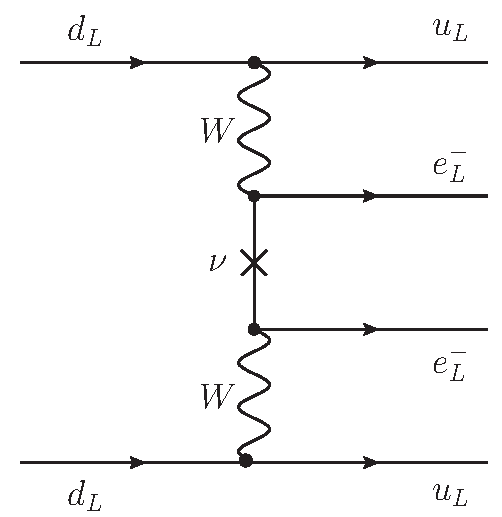
\includegraphics[scale=0.625]{img/LightNuExchange.pdf}
\caption{Neutrinoless double beta decay mediated by the standard mechanism, the virtual exchange of a light Majorana neutrino.} \label{fig:LightMajoranaNuExchange}
\end{figure}
%%%%%%%%%%

The standard mechanism responsible for the \bbonu\ decay is shown in Figure~\ref{fig:LightMajoranaNuExchange}.  The parent nucleus emits a pair of virtual $W$ bosons, and then these exchange a Majorana neutrino to produce the outgoing electrons. At the vertex where it is emitted, the exchanged neutrino is created, in association with an electron, as an antineutrino with almost total positive helicity, and only its small, $\mathcal{O}(m_{\nu}/E)$, negative-helicity component is absorbed at the other vertex. Considering that the amplitude is, in this case, a sum over the contributions of the three light neutrino mass states $\nu_i$ and is proportional to the square of the elements of the neutrino mixing matrix, $U_{ei}^2$, we conclude that the modulus of the amplitude for the \bbonu\ process must be proportional in this case to the \emph{effective neutrino Majorana mass}:
%%%
\begin{equation}
\mbb \equiv \left|\, \sum_{i=1}^3 U_{ei}^2\cdot m_i\ \right|, \label{eq:mbb}
\end{equation}
%%%
where $U_{ei}$ are the elements of the first row of the neutrino mixing matrix and $m_{i}$ are the three neutrino masses.

In the case where light Majorana neutrino exchange is the dominant contribution to \bbonu-decay, the inverse of the half-life for the process can be written as
%%%
\begin{equation}
\left(T^{0\nu}_{1/2}\right)^{-1} = G^{0\nu}\ \left|M^{0\nu}\right|^2\ \left(\frac{\mbb}{m_{e}}\right)^2.
\label{eq:Tonu}
\end{equation}
%%%
Here, \Gonu\ is a phase-space factor that depends on the transition $Q$ value and on the nuclear charge $Z$, and $M^{0\nu}$ is the nuclear matrix element (NME) for the process. The phase-space factor can be calculated analytically with sufficient accuracy (error estimates of about 1 per mille). The NME is evaluated using nuclear models, although with considerable uncertainty. In other words, the value of the effective neutrino Majorana mass, \mbb, can be inferred from a non-zero \bbonu-rate measurement, even though with some nuclear physics uncertainties. Conversely, if a given experiment does not observe the \bbonu\ process, the result can be interpreted in terms of an upper bound on \mbb.  

%%%%%%%%%%
\begin{figure}
\centering
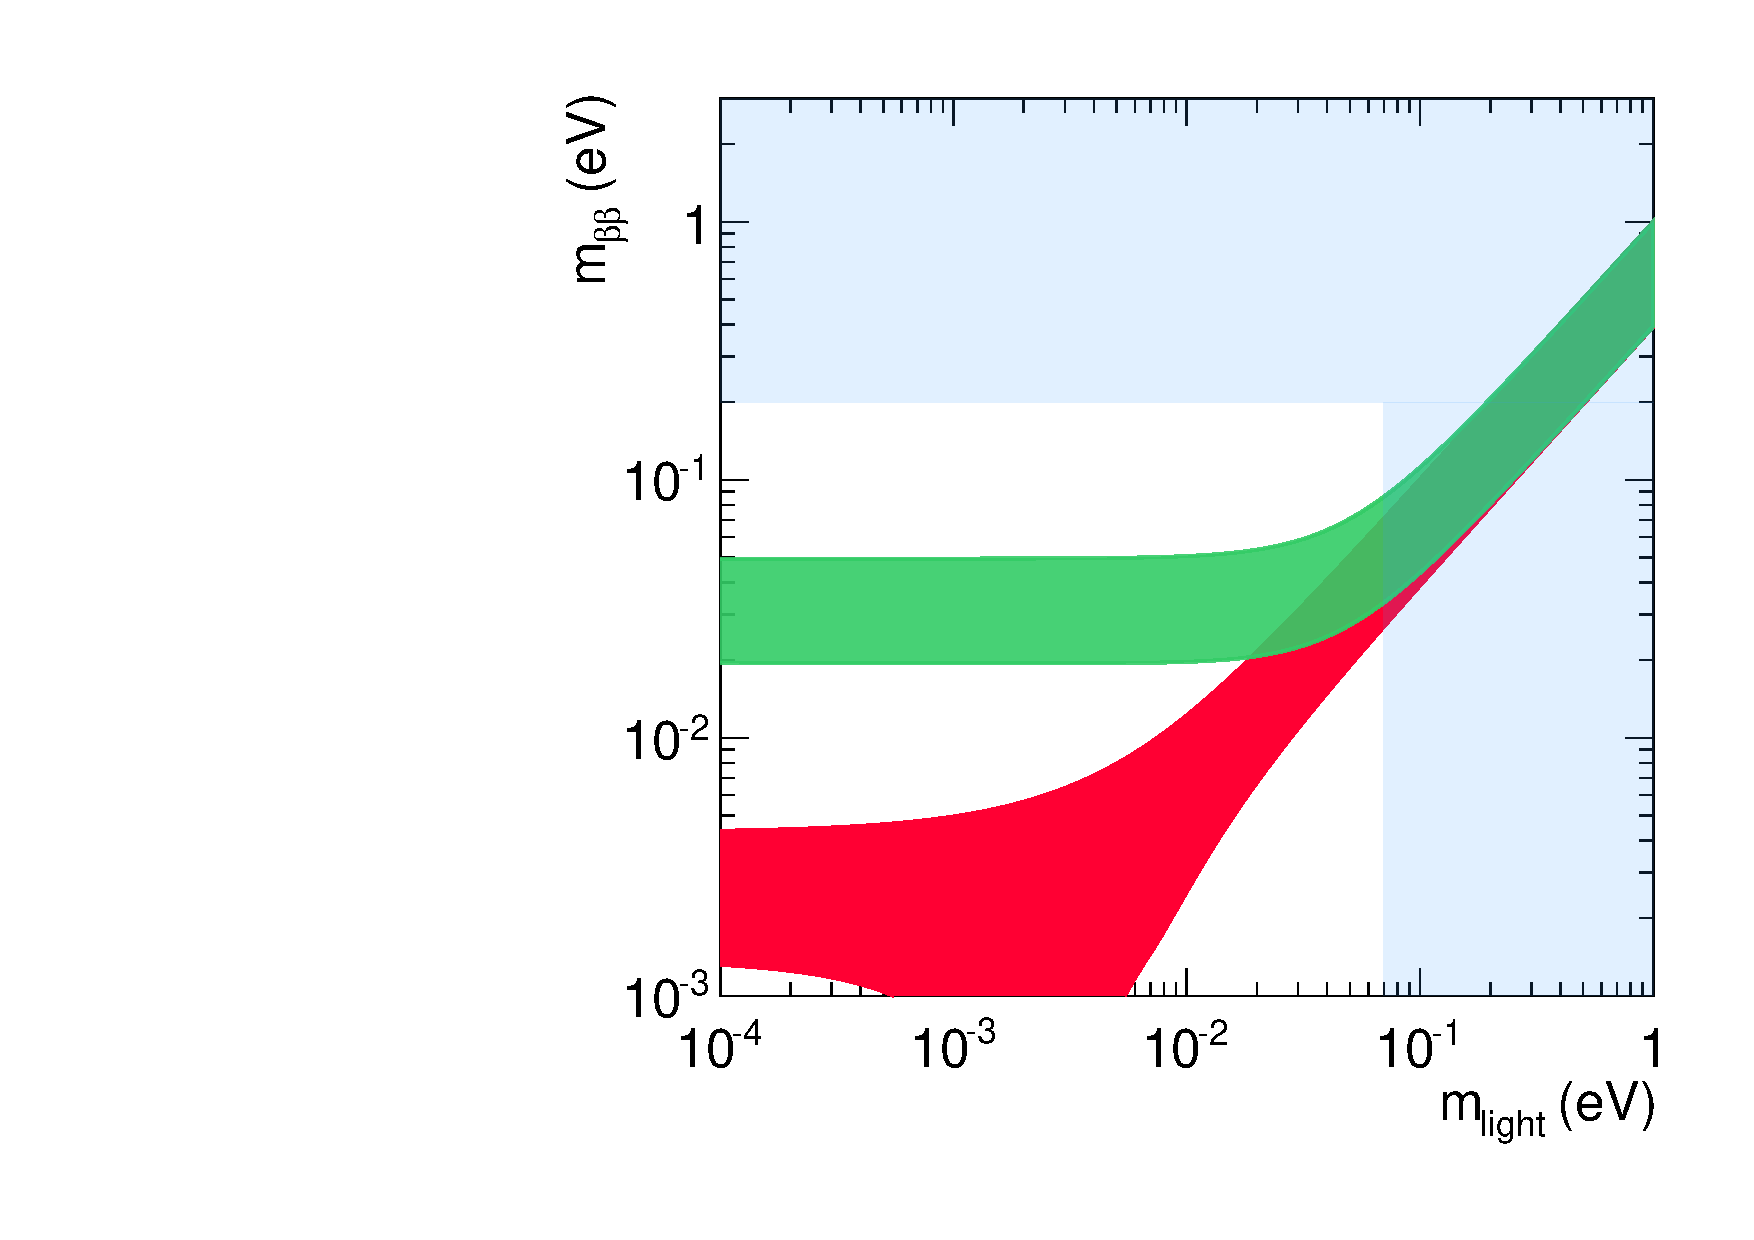
\includegraphics[width=0.525\textwidth]{img/BetaBetaVsLight.pdf}
\caption{The effective neutrino Majorana mass, \mbb, as a function of the lightest neutrino mass, $m_\mathrm{light}$. The green band corresponds to the inverted ordering of neutrino masses ($m_\mathrm{light}\equiv m_{3}$), while the red band corresponds to the normal ordering ($m_\mathrm{light}\equiv m_{1}$). The vertically-excluded region comes from cosmological bounds, while the horizontal one from \bbonu\ constraints.} \label{fig:BetaBetaVsLight}
\end{figure}


If light Majorana neutrino exchange is the dominant mechanism for \bbonu\ decay, it is clear from Eq.~(\ref{eq:mbb}) that the decay is then directly connected to neutrino oscillations phenomenology, and that it also provides direct information about the absolute neutrino mass scale. The relationship between \mbb\ and the actual neutrino masses $m_i$ is affected by the uncertainties in the measured oscillation parameters, the unknown neutrino mass ordering (normal or inverted) and the unknown phases in the neutrino mixing matrix (both Dirac and Majorana). For example, the relationship between \mbb\ and the lightest neutrino mass, $m_\mathrm{light}$, is shown in Figure~\ref{fig:BetaBetaVsLight}. The width of the two bands is due to the unknown CP violation phases and the uncertainties in the measured oscillation parameters. Figure \ref{fig:BetaBetaVsLight} also shows the upper bound on $m_\mathrm{light}$ from cosmology ($m_\mathrm{light}<0.07$ eV ), and an upper bound on \mbb\ from the current generation of \bbonu-decay searches ($m_{\beta\beta}<0.2$ eV ). See \cite{Gomez-Cadenas:2015twa} for a more detailed discussion and a full list of references). 

Notice that the current bounds on \mbb\ derived from GERDA-I, EXO-200 and KamLAND-ZEN, are of the order of $\mbb < 200$~meV, while the cosmological bounds on m$_{light}$~are of the order of
$m_{light} < 100$~meV. By $\sim$ 2020, The ``current generation'' of \bbonu\ experiments (including GERDA-II, {\scshape Majorana}, NEXT, CUORE, SNO+  and the SuperNEMO demonstrator, as well as upgrades of KamLAND-ZEN and EXO-200) will, probably, be able to push the current sensitivity to about $\mbb < 50-100$~meV. If a discovery is not made, then, the current generation of \bbonu\ experiments will exclude the so-called ``degenerated hierarchy'' ($m_1 \sim m_2 \sim m_3$) of neutrino masses. The goal of the ``next generation'' of \bbonu\ experiments is to fully explore the inverse hierarchy (green band in the figure, $\mbb < 20$~meV.)

%%%%%%%%%%
